%% Autor: Björn Ritterbecks 
%% Letzte Aenderung: 15.06.2016 
\thisfloatsetup{%
  capbesidewidth=\marginparwidth}
\begin{figure}[htbp]
\centering
%\sansmath
 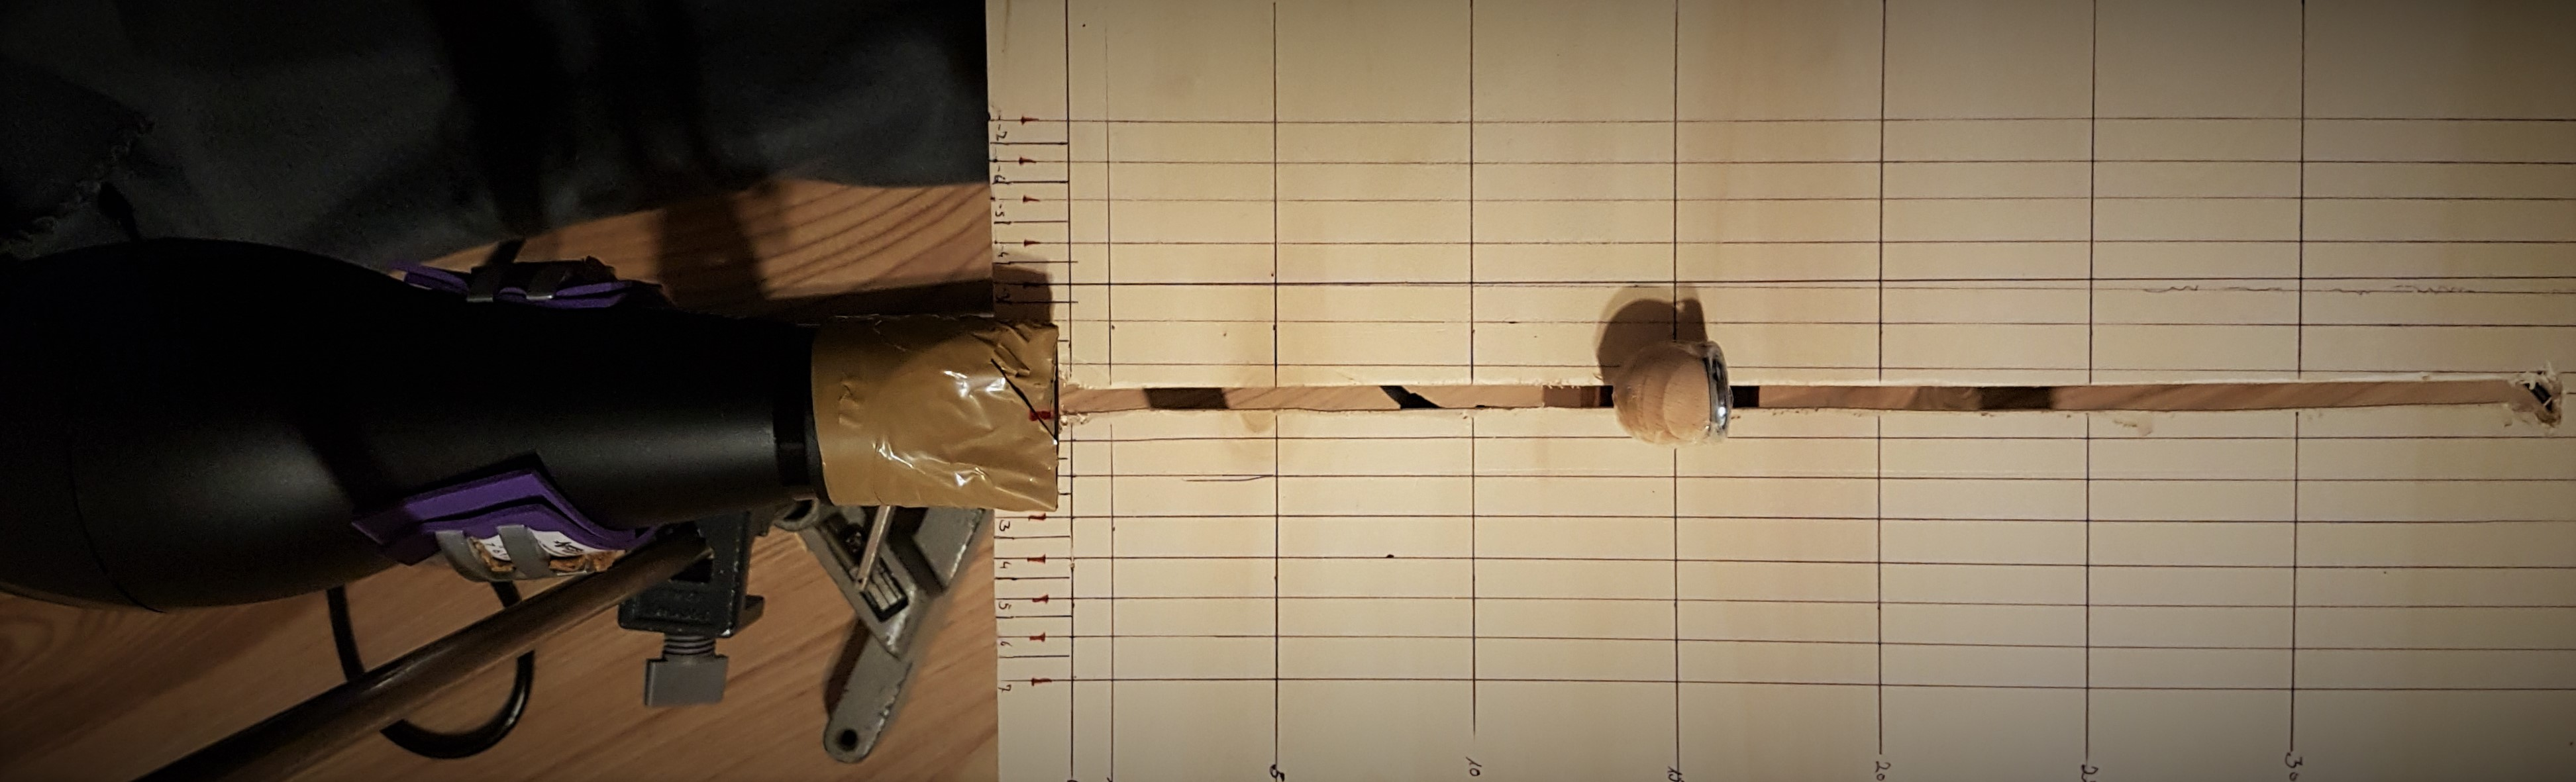
\includegraphics[width=0.99\textwidth]{images/stroemungskraftmessung4.jpg}
  \caption[Zweiter Versuchsaufbau zur Srömungskraftmessung]{Draufsicht des zweiten Versuchsaufbaus für die Messungen zur Strömungswiderstandskraft von Kugeln unterschiedlicher Radien. Ein Föhn ist beweglich auf einem Stativfuß an dem Messtisch angebracht, der mit einem Koordinatensystem für die Messreihen präpariert ist.}
  \label{fig:stroemungskraftmessung4}
  \vspace{-0pt}
\end{figure}